\section*{Figures}

%Figures should be uploaded as a separate file (or files) as .jpg or .tif files.

%Full instructions on preparing the figures are available as part of the online submission instructions. Please follow these instructions carefully as failure to do so will delay publication of your manuscript (please note: the editors reserve the right to charge for extensive changes).
%In preparing graphs authors should avoid background tints and 3D effects and maintain a consistent label size and aspect ratio (the x/y axis ratio) throughout a paper. Figure and axes titles should be clear and NOT in bold text. Do not include more figures than is absolutely necessary - non-essential figures may be judged as being suitable for online-only publication.

\begin{figure}[ht]
\centering
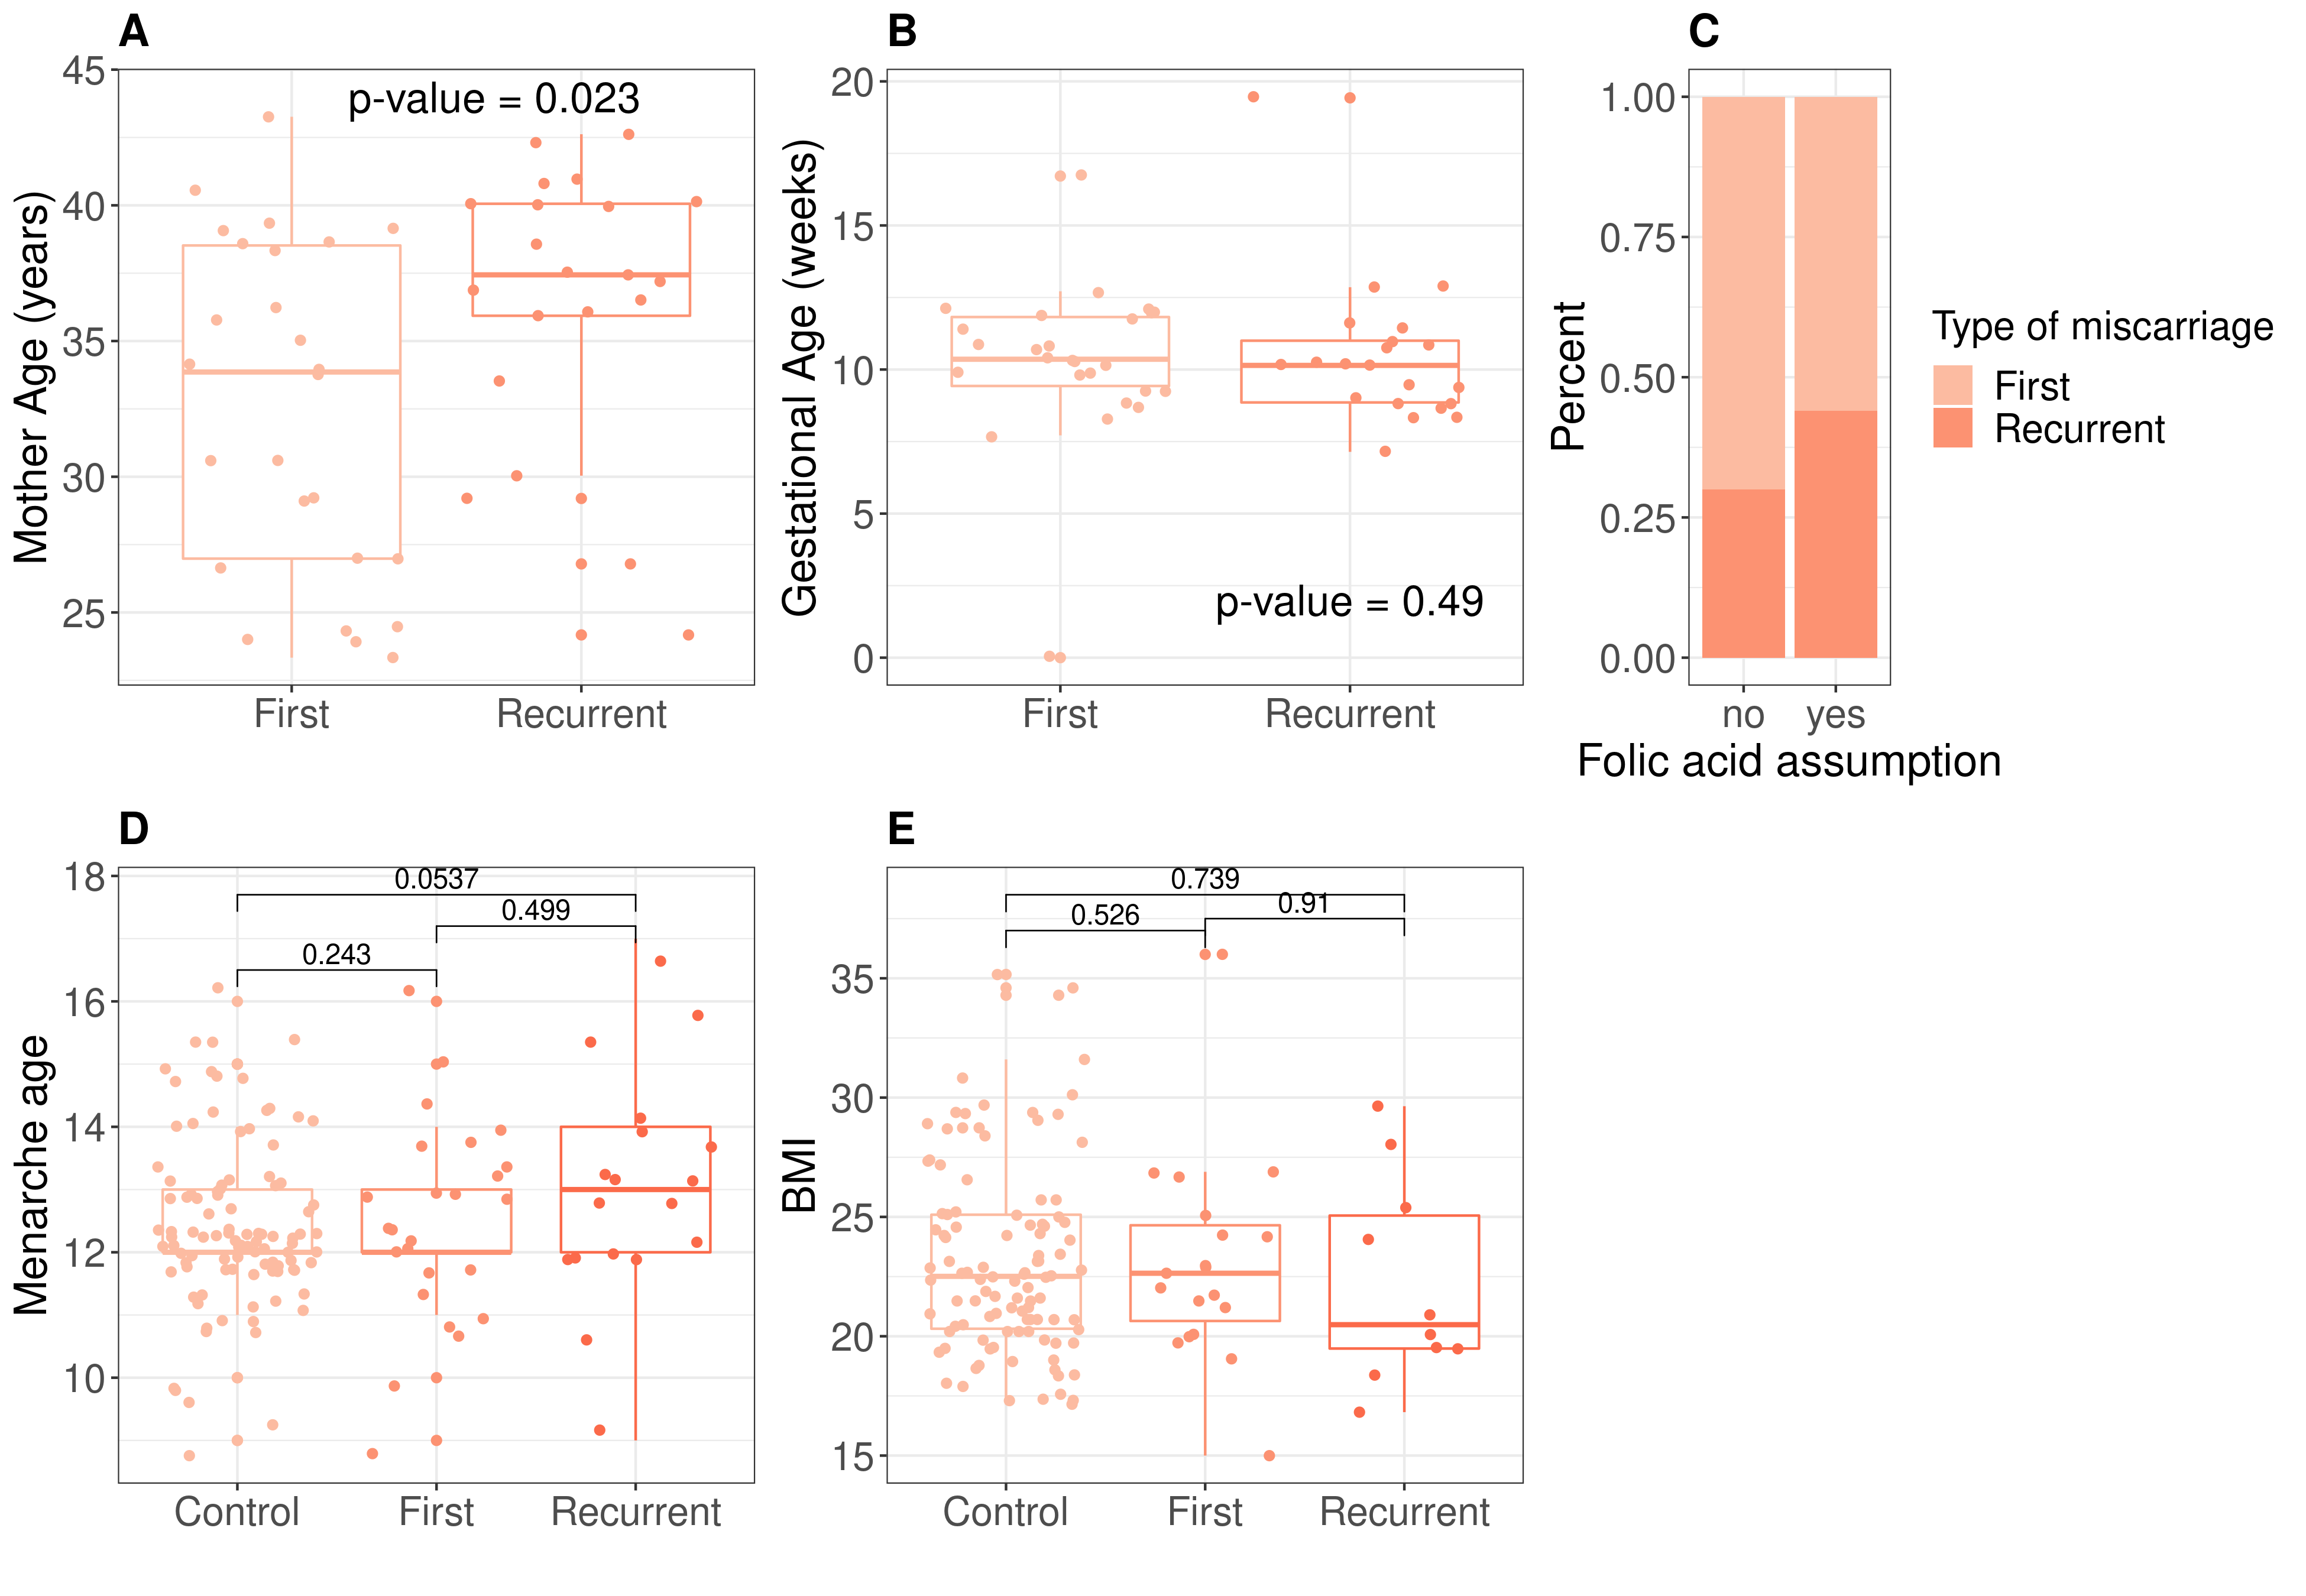
\includegraphics[width=\linewidth]{fig/panel_stats.png}
\caption{\textbf{Features of the embryo's mothers.} \textbf{(A)} Median age of the mother at the event is XX and XX for first and recurrent miscarriages, with no significant difference. \textbf{(B)} Gestational age at the time of the pregnancy termination range from X to X weeks with no significant difference between first and recurrent cases.  \textbf{(C)} Folic acid intake. Range of values of menarche age \textbf{(D)} and Body Mass Index \textbf{(E)} in embryo's mothers are not significantly different from a control set of mothers undergoing voluntary termination of pregnancy.}
\label{fig:embryostats}
\end{figure}

\begin{figure}[h]
\centering
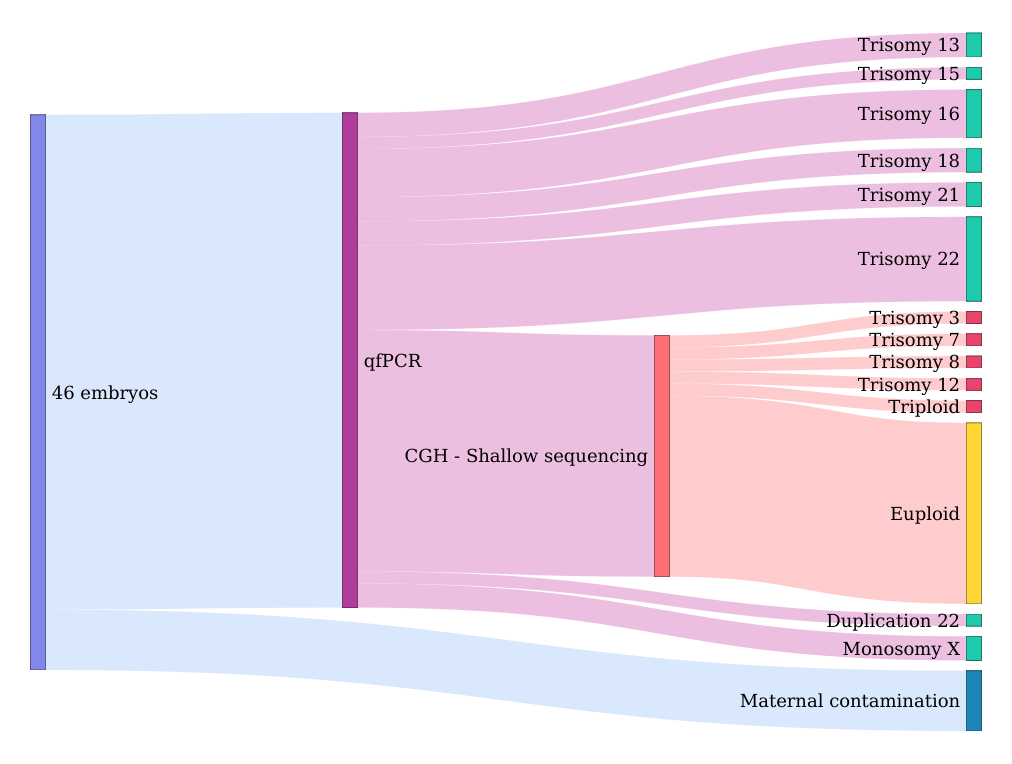
\includegraphics[width=0.7\textwidth]{fig/ibelieve.png}
\caption{\textbf{Outcome of the screening for aneuploidies in the embryos.} Forty-six embryos were screened by quantitative PCR to determine aneuploidies of chromosomes 13, 15, 16, 18, 21, 22, X, and Y, as well as to determine maternal contamination. DNA of embryos with no anuploidies in these chromosomes were further analyzed by comparative hybridization and shallow sequencing. Overall we found aneuploidies in  56.6\% of the embryos, the most common being the trisomy of chromosome 22. In yellow the fraction of euploid embryos. }
\label{fig:presequencing}
\end{figure}

\begin{figure}[ht]
\centering
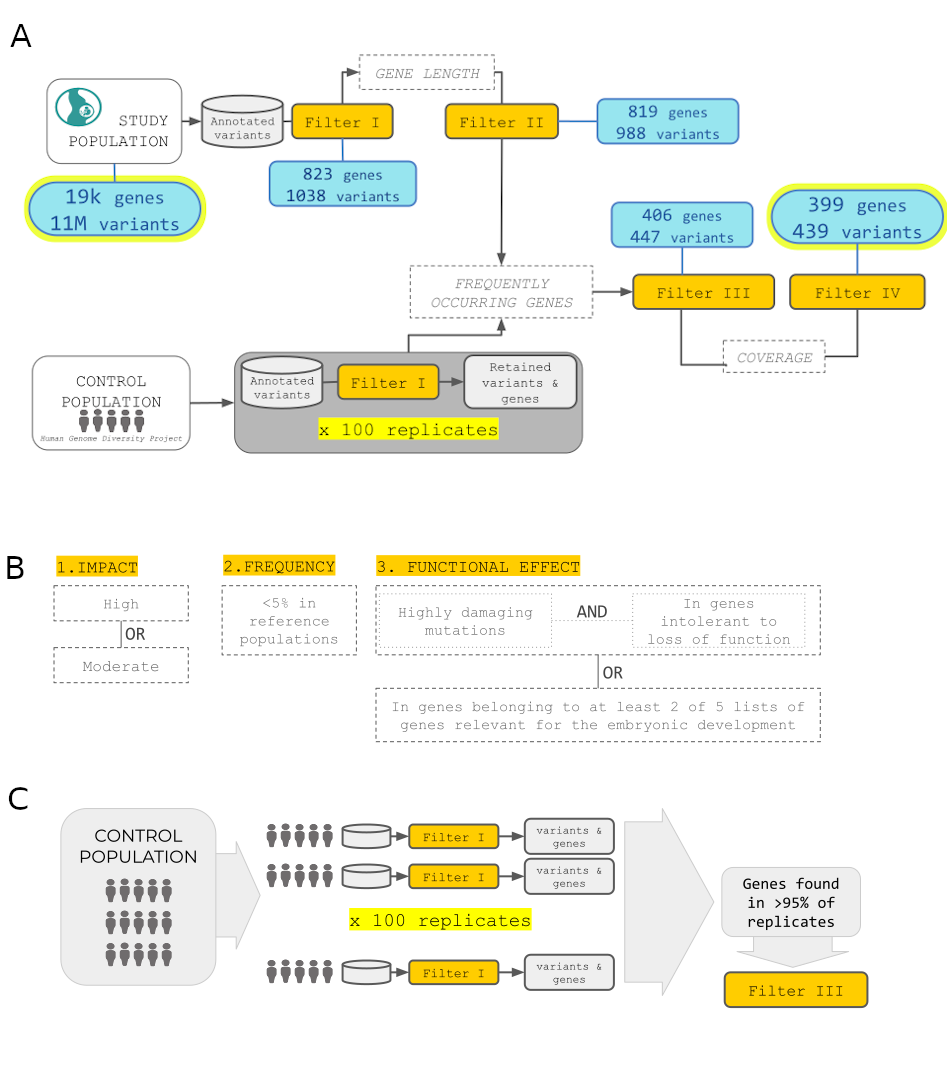
\includegraphics[width=\linewidth]{fig/pipe.png}
\caption{\textbf{Overview of the pipeline for prioritization of the genetic variants.} \textbf{(A)} \gp takes as input genomic variants information from cases and controls and outputs a subset of variants prioritized according to user-defined parameters \gp currently analyzes coding regions and performs four filtering steps. \textbf{(B)} Filter I retains variants based on three criteria: overall impact on the gene product moderate or high, allele frequency in control populations, the combined property of being putatively damaging (quantified bythe CADD score) and located in genes intolerant to loss of function (determined by the pLIscore). It is also possible to incorporate one or more user-defined lists of genes relevant to the trait under study. \textbf{(C)} Filter III determines the chance for genes to be selected in a control population based on criteria specified in Filter I. In practice, a number of control individuals are sampled a number of times and their genetic data filtered using Filter I to obtain a list of genes selected by chance.} 
\label{fig:pipeline}
\end{figure}
%Genetic variants discovered in samples and controls are annotated and Filtered on the basis of the annotations (Filter I). In samples  Samples are first screened for the quality of DNA and maternal contamination and then analyzed for aneuploidies. \textbf{(B) Outcomes of the pipeline.} We estimate that 18\% of samples goes to sequencing....


\begin{figure}[ht]
\centering
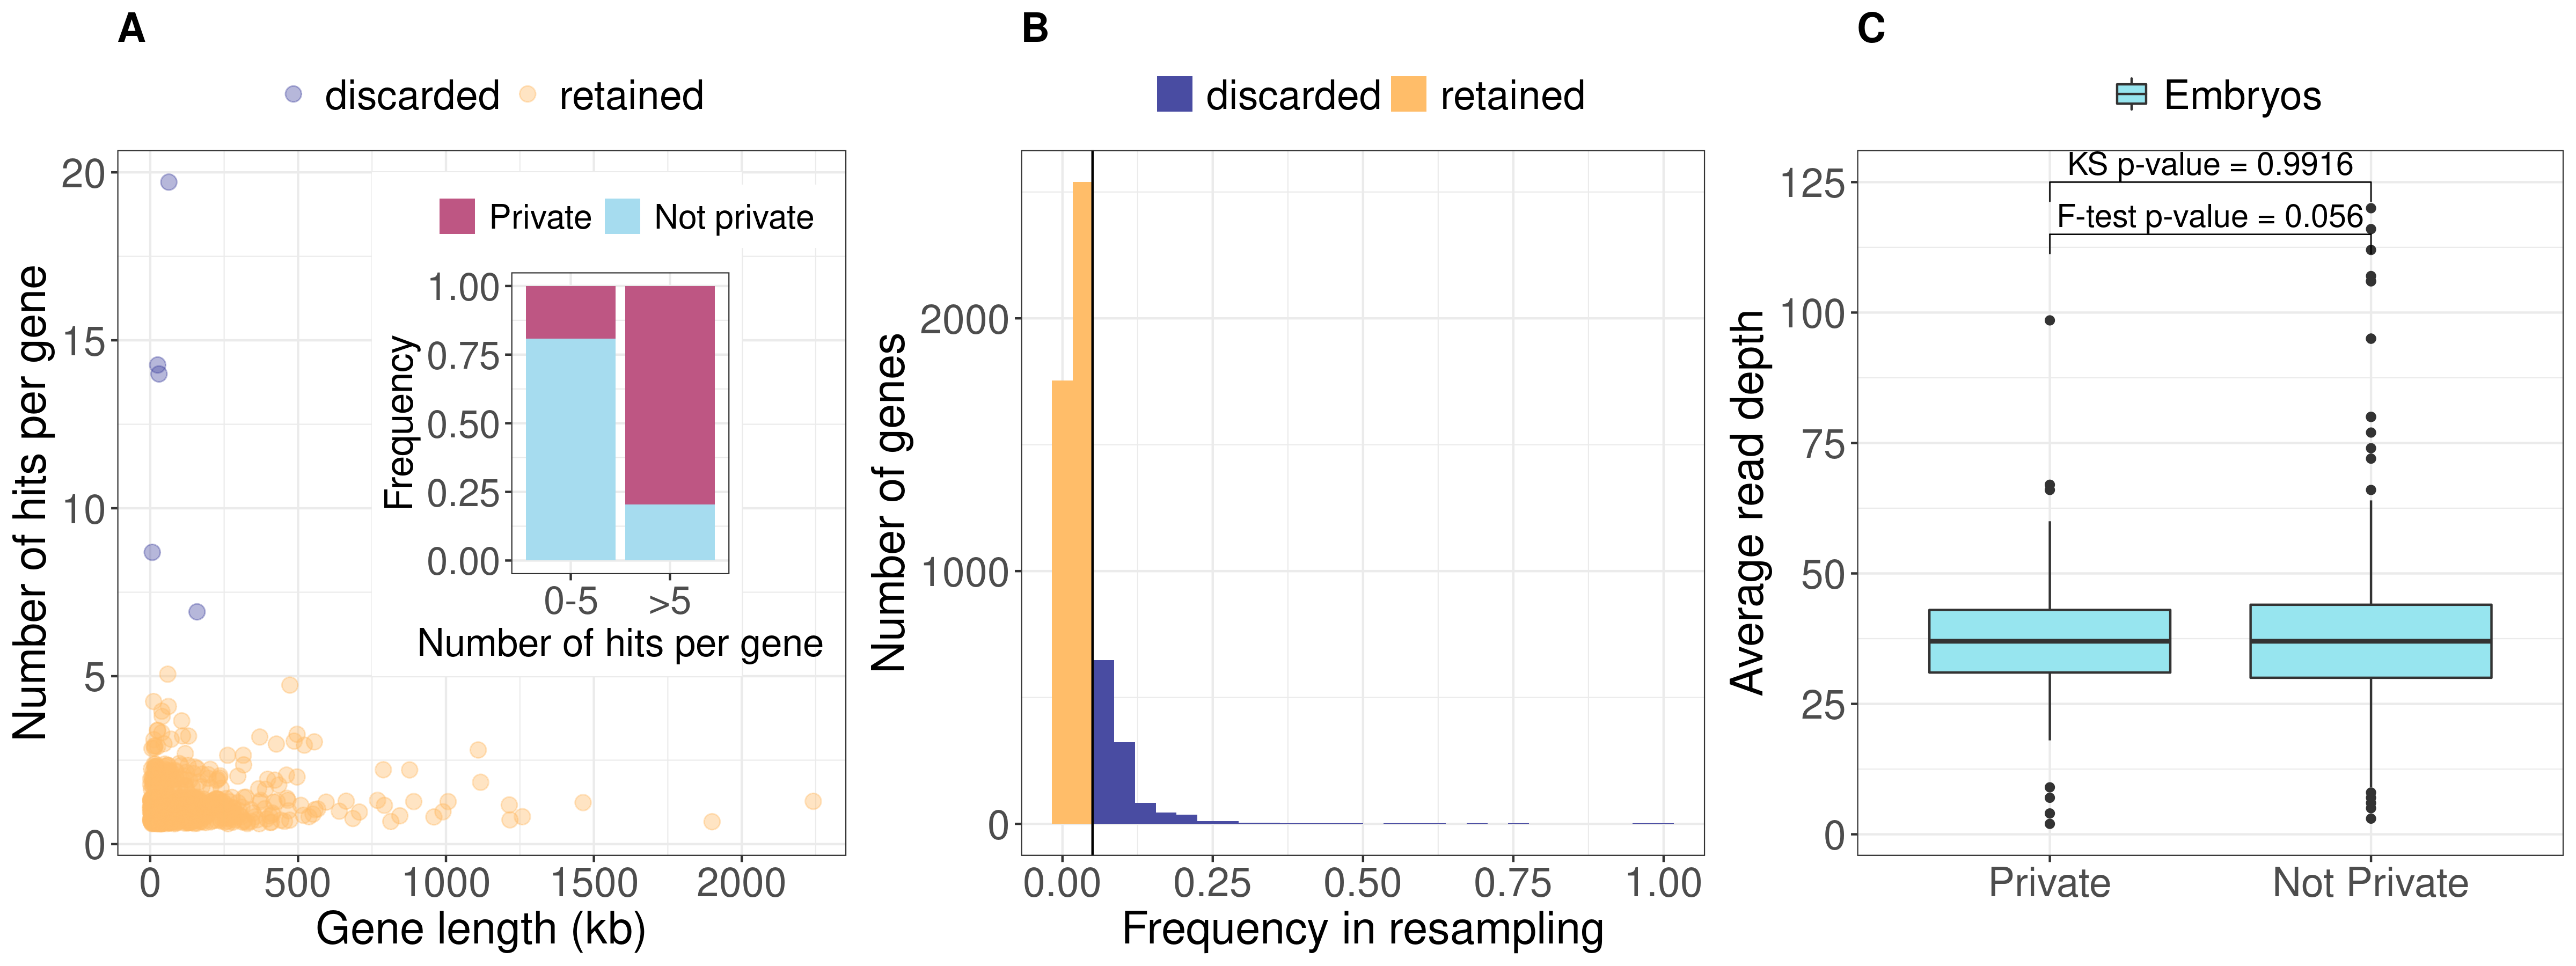
\includegraphics[width=\linewidth]{fig/filters_embryos.png}
\caption{\textbf{} \textbf{(A)} Number of hits per gene after Filter II. The majority of genes have less than five hits and there is no significant correlation between number of hits and gene length (Spearman r=0.05 p-value=0.124). In the insert: the genes with $>$5 hits are enriched for private variants. \textbf(B) Frequency across 100 replicates of genes that pass Filter I in resampling form a control population. Most genes are retained $<$5\% of times (yellow) therefore are retained if found in the embryos. 1,531 genes are instead retained in $>$5\% of replicates (blue) and therefore discarded if found in the embryos, under the assumption that they can be filtered by chance in healthy controls. \textbf{(C)} Despite comparable read depth between private and non-private variants After Filter III to control for possible artifacts due to scanty coverage, we further filter to remove hits that are private and with read depth outside the range found in non-private ones.}
\label{fig:filters}
\end{figure}

\begin{figure}[ht]
\centering
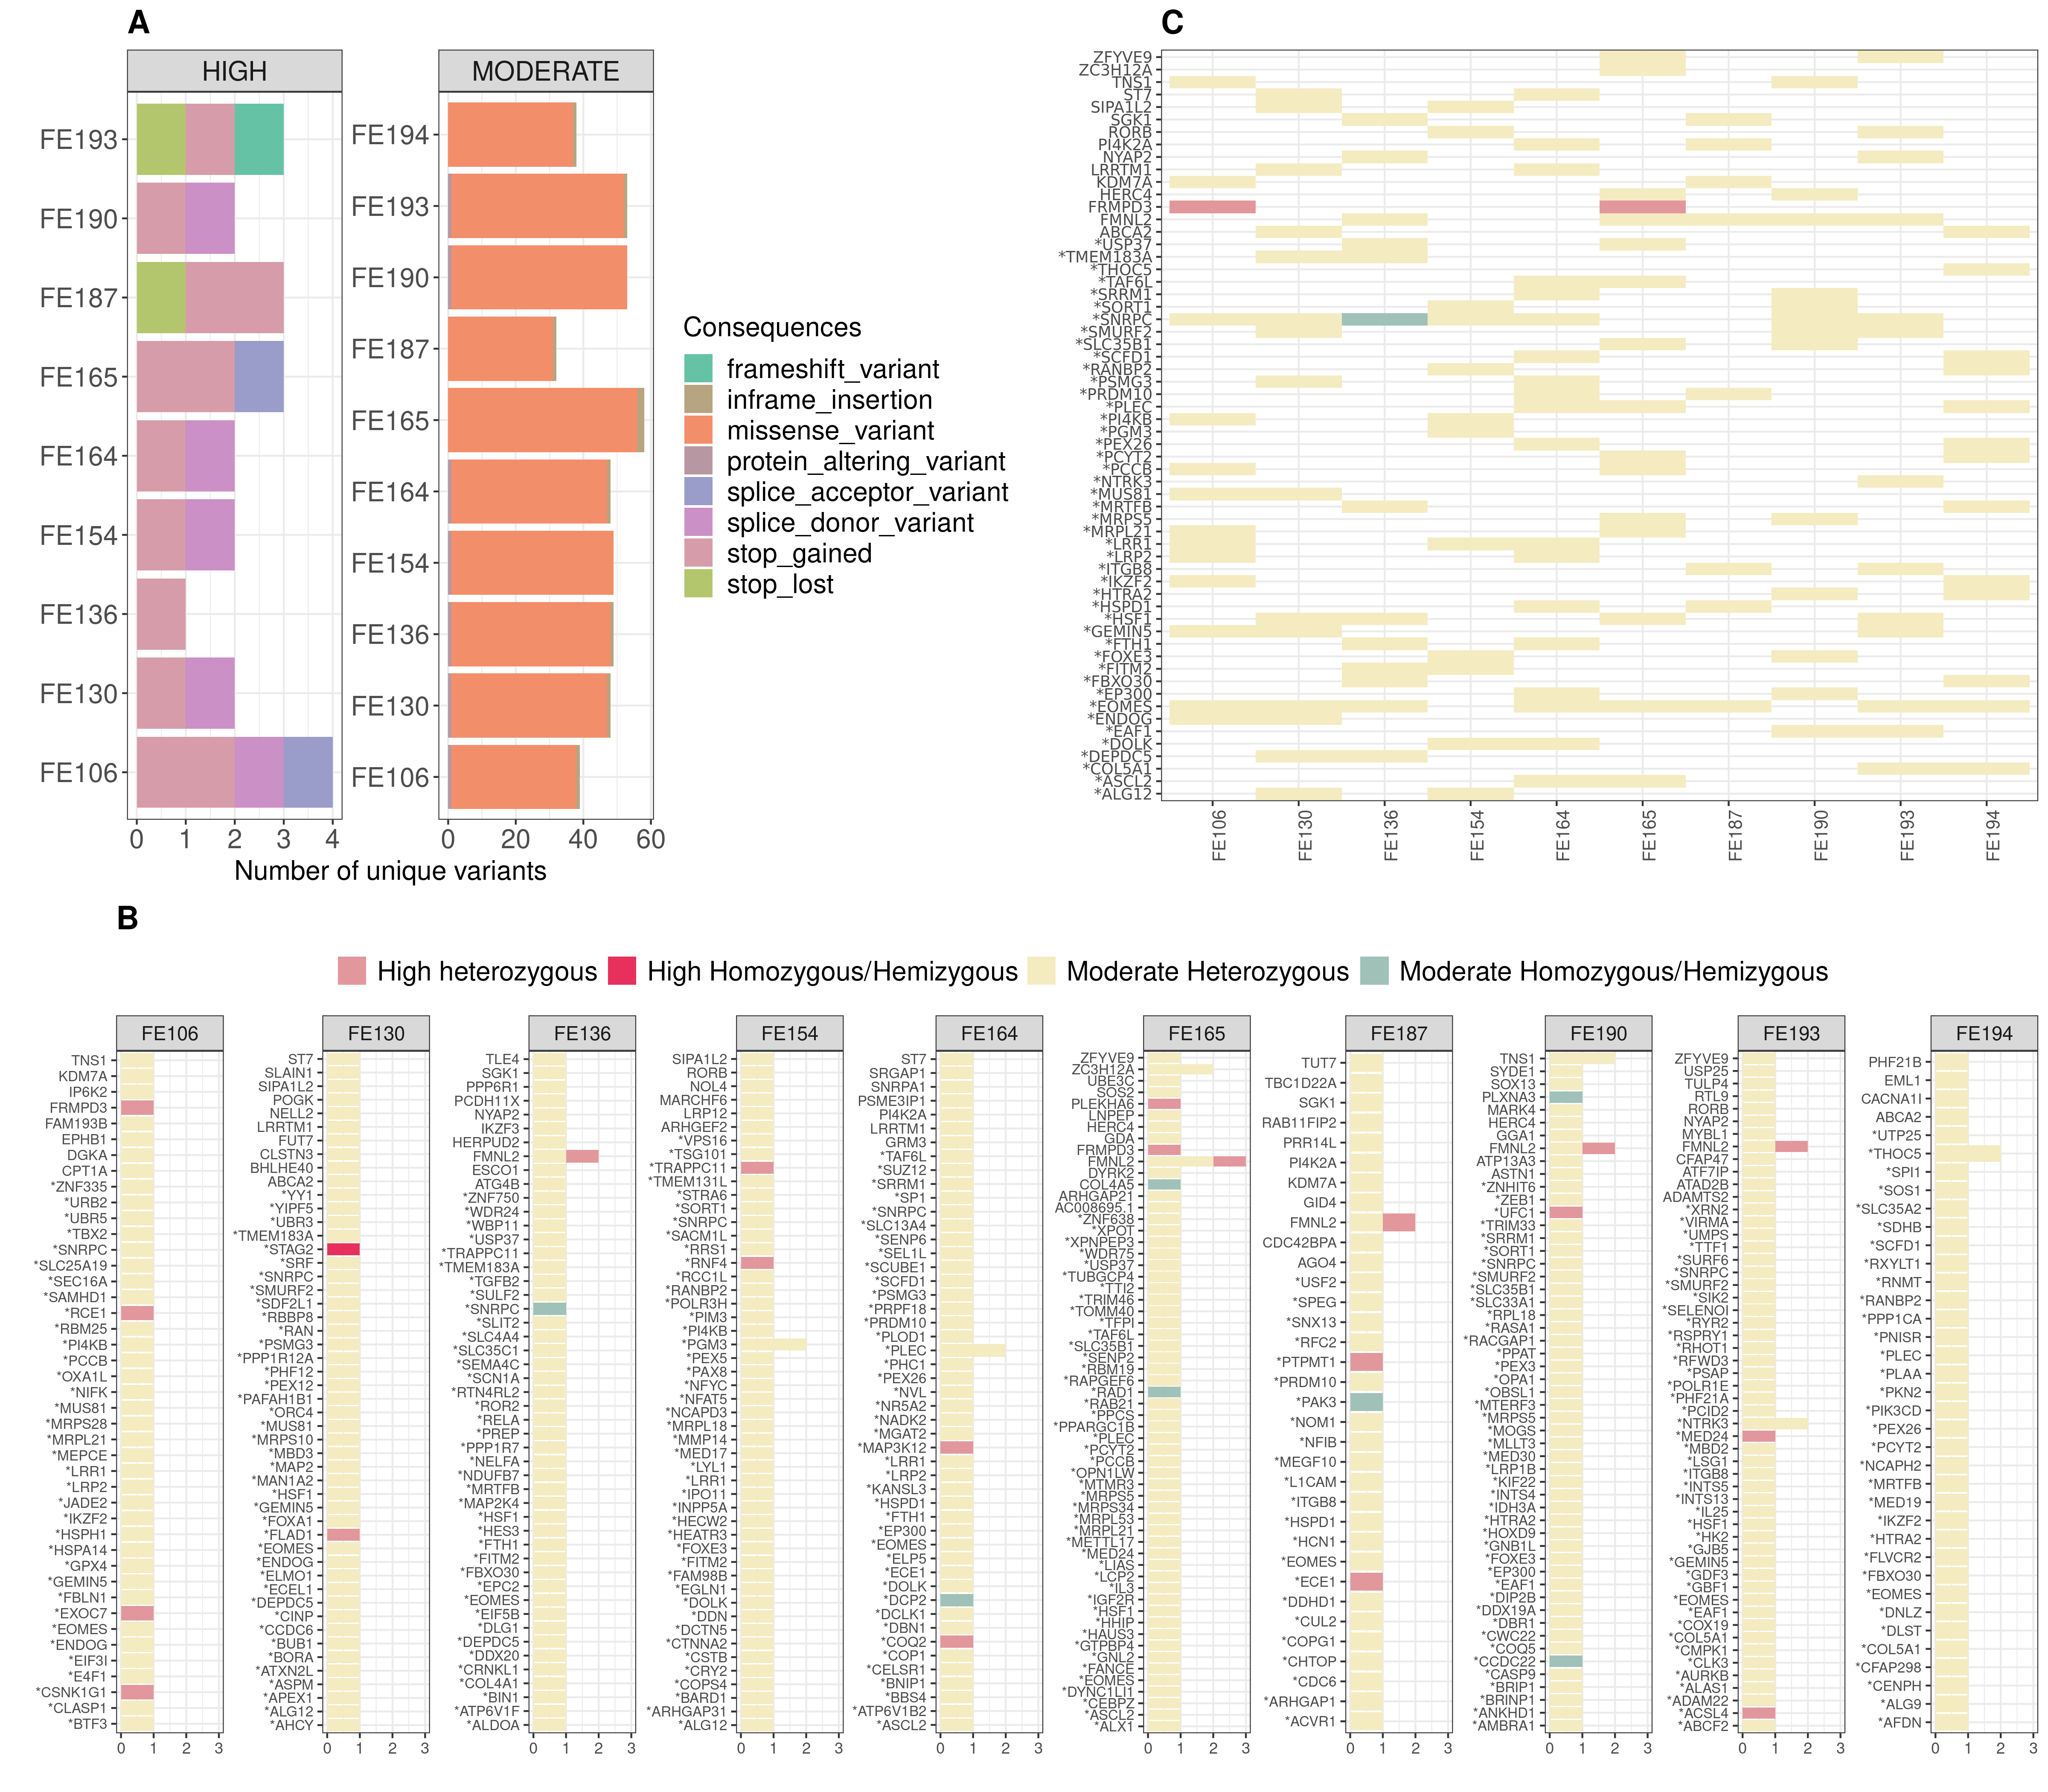
\includegraphics[width=\linewidth]{fig/panel_EmbryoResults.png}
\caption{\textbf{Results of the prioritization pipeline. (A)} Number of variants per embryo stratified by impact. Overall 4.1\% of the prioritized variants are classified as having high impact on the gene products. \textbf{(B)} Results per embryo. On the y-axis the prioritized genes while on the x-axis the number of mutations per gene. Colors indicate the allele count and the class of severity. \textbf{(C)} Selection of prioritized variants/genes shared by embryos.}
\label{fig:resembryo}
\end{figure}

\begin{figure}[ht]
\centering
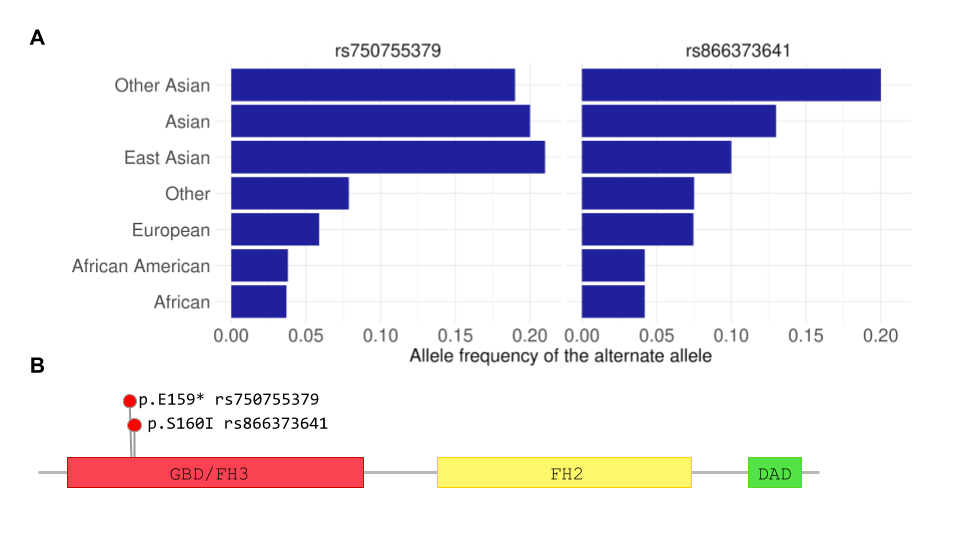
\includegraphics[width=\linewidth]{fig/fmnl2.png}
\caption{\textbf{Two-bases haplotype in \textit{FMNL2} prioritized in five embryos. (A)} Alelle frequencies from the NCBI Alpha database of the aternate alleles at rs750755379 and rs866373641. The two alleles exist at moderate-to high frequency in human populations. \textbf{(B)} Position in the protein of rs750755379 (stop gain) and rs866373641 (missense). The stop-gained mutation is located in the Rho GTPase-binding/formin homology 3 (GBD/FH3) domain involved in subcellular localization and regulation of activation. The resulting truncated protein lacks the Formin Homology-2 (FH2) domain, which directly binds to the actin filament catalyzing its nucleation and elongation. }
\label{fig:fmnl2}
\end{figure}